\documentclass[a4paper,12pt]{article}
\usepackage{graphicx} 
\usepackage{hyperref}
\usepackage{float}
\usepackage{amsmath}
\usepackage{enumitem}
\usepackage{amsfonts}
\usepackage{algorithm}
\usepackage{algorithmic}



% \begin{figure}[H]
%     \centering
%     \includegraphics[width=0.7\textwidth]{filename.png}
%     \caption{Your figure caption here.}
%     \label{fig:yourlabel}
% \end{figure}

\begin{document}

\title{Assignment 4 - Machine Learning \\
Theoretical Questions}
\author{Mohammad Hossein Basouli}
\date{\today}
\maketitle

\section*{Question 1}
\begin{enumerate}[label=(\alph*)]
    \item You have essentially removed the constraint for how great the magnitude of the parameters $\epsilon_i$'s can become. This causes the model to allow arbitrarily large errors, which leads to poor accuracy.
    \item I think so. If we set the $w$ such that its norm is so small, then the margin would be so large, but also we have to allow arbitrarily large errors $\epsilon_i$'s.
\end{enumerate}

\section*{Question 2}
\begin{enumerate}[label=(\alph*)]
    \item It controls the effect of linear terms over the other higher order terms. If we set $c = 0$, we have essentially removed the linear terms in our feature space, 
    whereas, if we set $c = 1$, we add linear terms based on our old feature space, to the new feature space. See the illustration in Figure~\ref{fig:fig_1}.
    \begin{figure}[H]
        \centering
        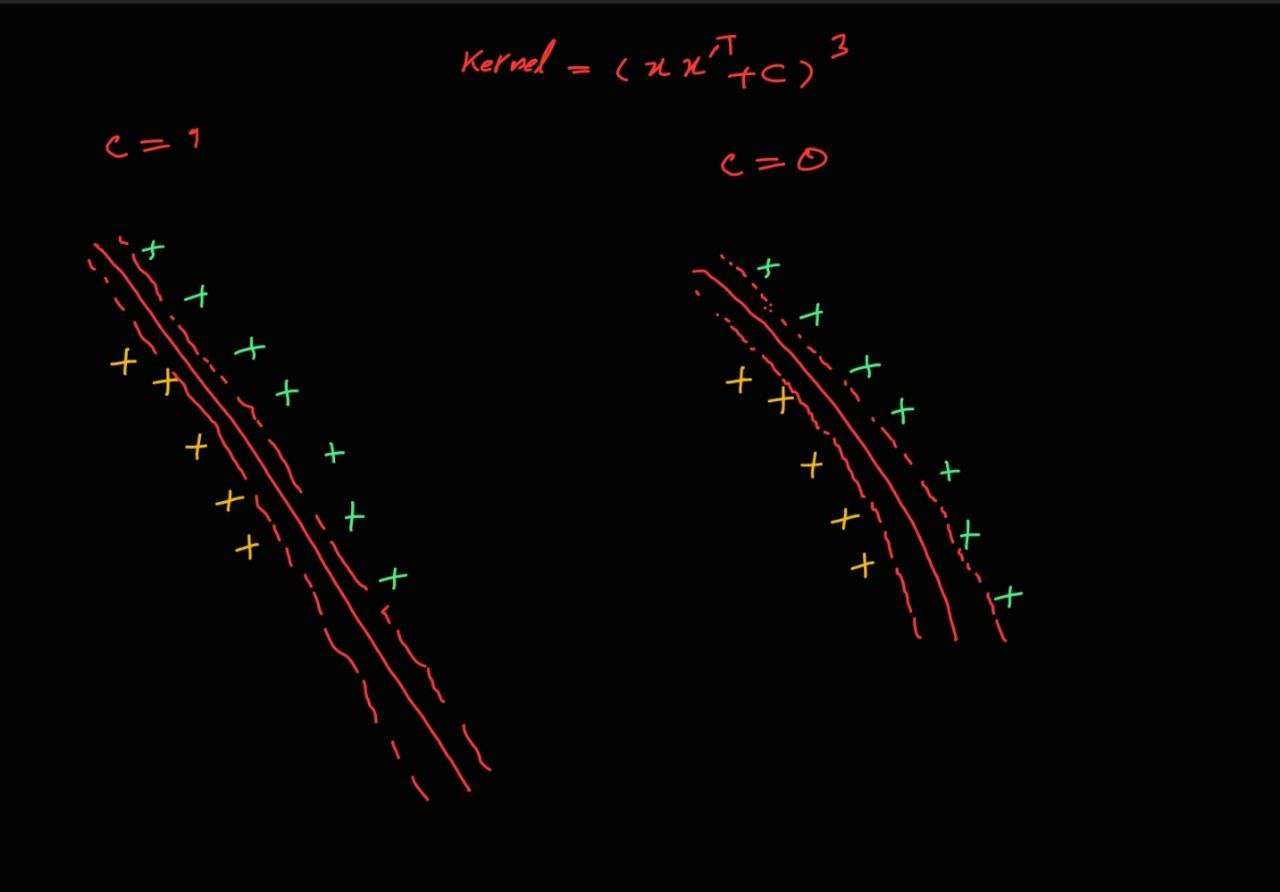
\includegraphics[width=0.7\textwidth]{../images/q2b.jpg}
        \caption{The figure illustrates the effect of inclusion and exclusion of constant term in the \textit{polynomial kernel}; 
        we can see that, by including the constant term (right section), the model has overfitted to the training data. 
        But in the left side, we can see a model which has the constant term excluded, which leads to a better fit.}
        \label{fig:fig_1}
    \end{figure}
    \item We can decrease both ($C$ and $\gamma$).
    \item Figure~\ref{fig:fig_2}
    \begin{align*}
    K(x, x') &= \exp\left(-\gamma \|x - x'\|^2\right) \\
    f(x) &= \sum_{i=1}^{n} \alpha_i y_i \exp\left(-\gamma \|x - x_i\|^2\right) + b \\
    \text{Solid lines (decision boundary):} &\quad f(x) = 0 \\
    \text{Dashed lines (margin boundaries):} &\quad f(x) = \pm 1
    \end{align*}
    \begin{figure}[H]
        \centering
        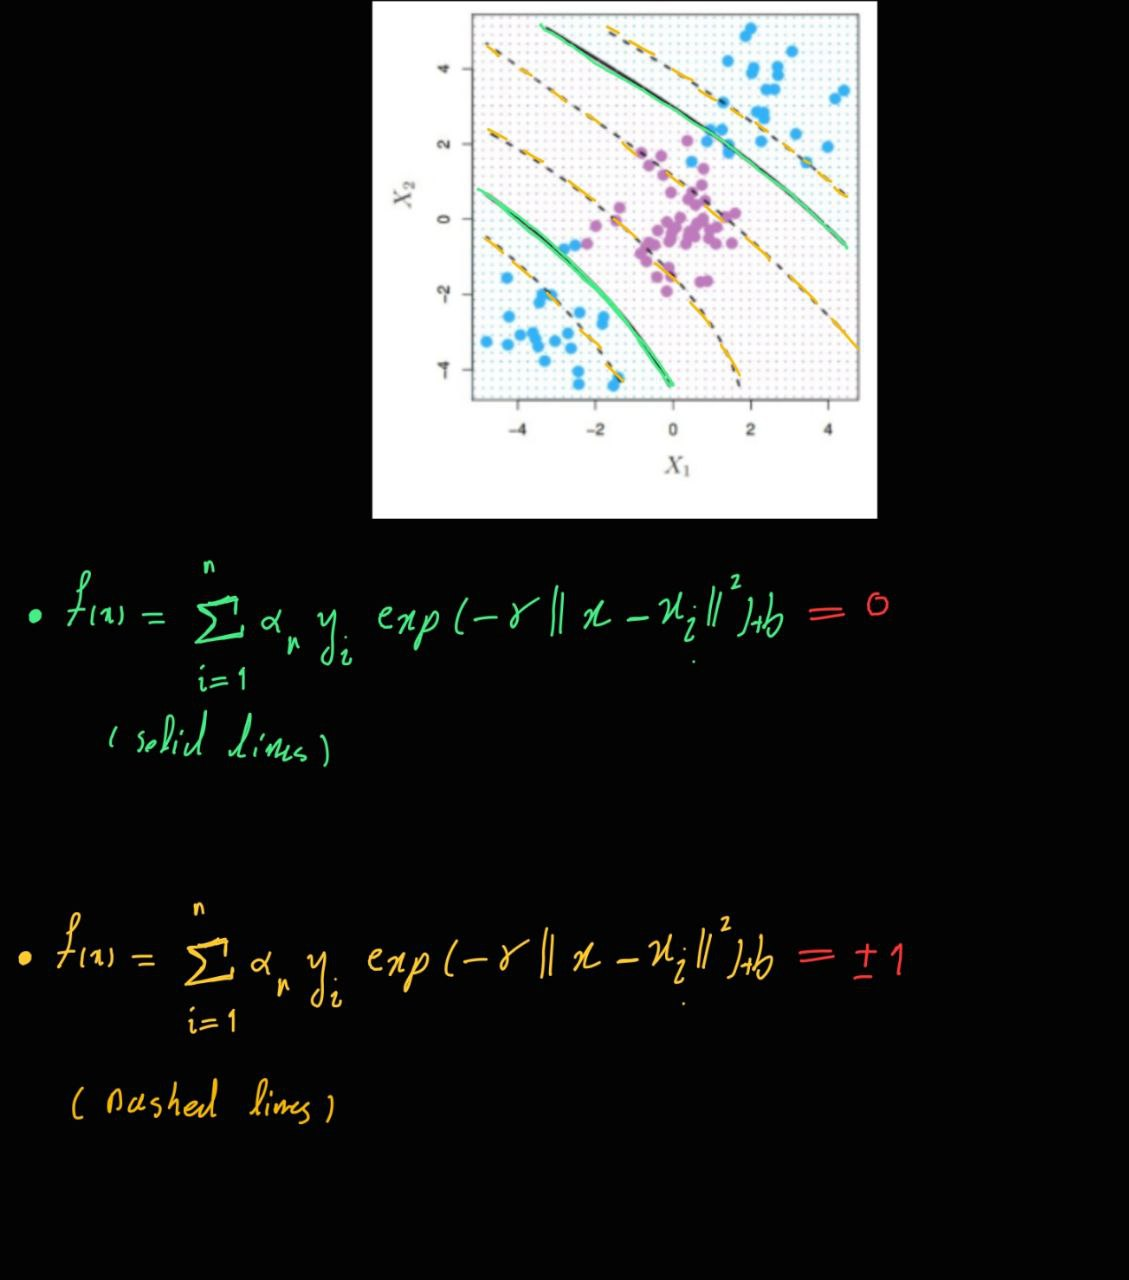
\includegraphics[width=0.7\textwidth]{../images/q2c.jpg}
        \caption{The figure shows the equation for solid and dashed lines in SVM using \textit{RBF kernel}.}
        \label{fig:fig_2}
    \end{figure}
\end{enumerate}

\section*{Question 3}
In pre-pruning, we prune the tree, as it grows by checking some criterion such as:
\begin{itemize}
    \item Is a minimum number of samples reached in a node?
    \item Is a maximum depth reached?
    \item Does Information Gain increase enough? 
\end{itemize}

Whereas in post-pruning, we prune the tree, after it has fully grown, by removing the splittings that add low to no true splitting in the data. Some of the methods for this are:
\begin{itemize}
    \item Reduced Errro Pruning
    \item Cost Complexity Pruning
\end{itemize}

\begin{table}[ht!]
\centering
\resizebox{\linewidth}{!}{%
\begin{tabular}{|l|c|c|}
\hline
\textbf{Aspect} & \textbf{Pre-Pruning} & \textbf{Post-Pruning} \\
\hline
Bias & High (due to early stopping) & Moderate (more flexible) \\
\hline
Variance & Lower (less overfitting) & Moderate (prunes overfit tree) \\
\hline
Computational Cost & Lower (stops tree early) & Higher (full growth + pruning) \\
\hline
\end{tabular}%
}
\caption{Comparison of Pre-Pruning and Post-Pruning}
\end{table}

\section*{Question 4}
Yes, the Gini impurity of an individual child node can be greater than that of its parent. However, the weighted average of the child nodes' Gini impurities will always be less than or equal to the Gini impurity of the parent node.
\textbf{Parent Node:}

Class A: 30, \quad Class B: 20

\[
p_A = \frac{30}{50} = 0.6, \quad p_B = 0.4
\]

\[
\text{Gini}_{\text{parent}} = 1 - (0.6^2 + 0.4^2) = 1 - (0.36 + 0.16) = 0.48
\]

\vspace{1em}
\textbf{After Split:}

\textbf{Left Child:}

Class A: 20, \quad Class B: 10

\[
p_A = \frac{20}{30} \approx 0.67, \quad p_B \approx 0.33
\]

\[
\text{Gini}_L = 1 - (0.67^2 + 0.33^2) \approx 1 - (0.4489 + 0.1089) = 0.4422
\]

\textbf{Right Child:}

Class A: 10, \quad Class B: 10

\[
p_A = p_B = 0.5
\]

\[
\text{Gini}_R = 1 - (0.5^2 + 0.5^2) = 1 - (0.25 + 0.25) = 0.5
\]

\vspace{1em}
\textbf{Weighted Gini after split:}

\[
\text{Gini}_{\text{split}} = \frac{30}{50} \cdot 0.4422 + \frac{20}{50} \cdot 0.5 = 0.264 + 0.2 = 0.464
\]

\textbf{Conclusion:} Even though \( \text{Gini}_R > \text{Gini}_{\text{parent}} \), the overall weighted Gini impurity decreased: \( 0.464 < 0.48 \).

\section*{Question 5}
Figure~\ref{fig:fig_3}
\begin{figure}[H]
    \centering
    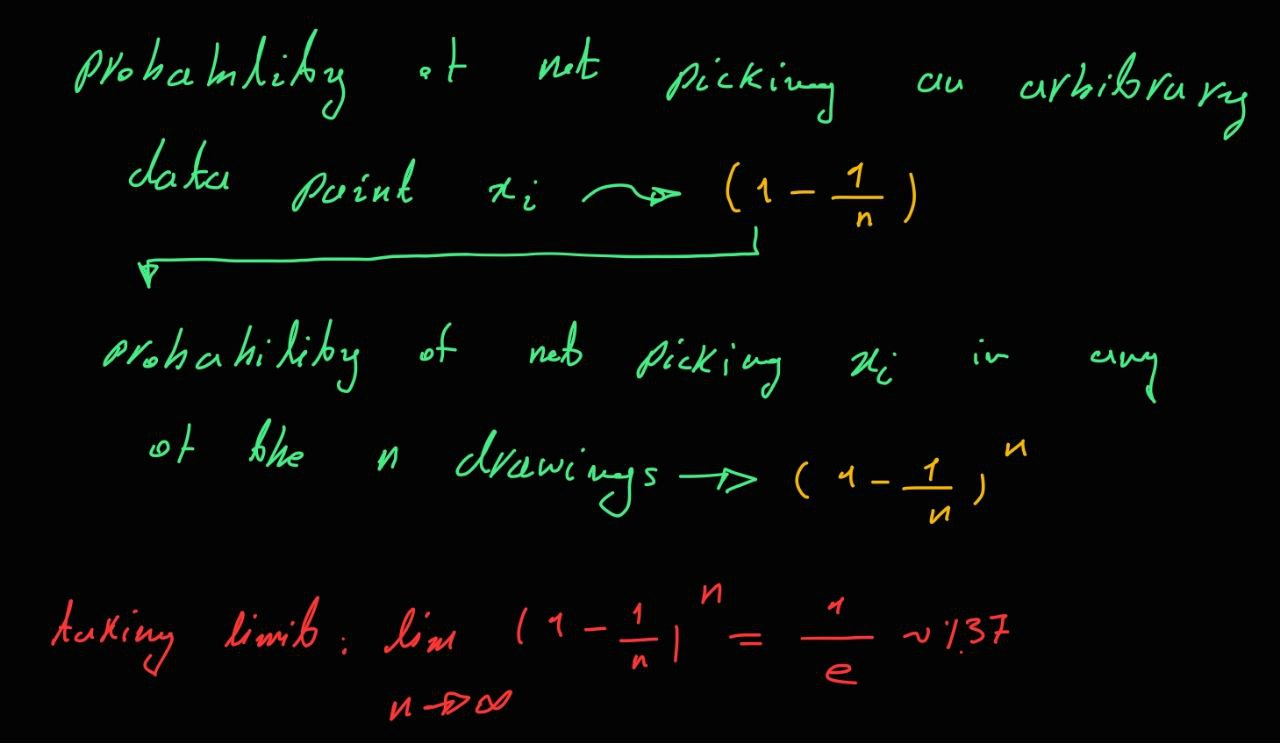
\includegraphics[width=0.7\textwidth]{../images/q5.jpg}
    \caption{Justification for why, each bootstrapped dataset contains only 63 percent of the original samples.}
    \label{fig:fig_3}
\end{figure}

\section*{Question 6}

\noindent\textbf{AdaBoost} in Short: AdaBoost first gives equal weights to each of the samples in the dataset, and then tries to fit the best stump to the data. 
Then it calculates the errors and updates the weights for each of the samples, based on how much error the model has made for that sample. Next, 
it will calculate how much error the model has made overall to give the model's prediction a weight. And it repeats the process for a certain number of iterations and then sum them up.

\noindent\textbf{Gradient Boosting} in Short: Unlike AdaBoost, in Gradient Boosting, instead of assigning weight to the data points, we will use the negative of the gradient of the loss function to 
build new models that correct the previous errors, made by the older models. 

\begin{algorithm}
\caption{AdaBoost Algorithm}
\begin{algorithmic}[1]
\REQUIRE Training set $\{(x_1, y_1), \dots, (x_n, y_n)\}$ with $y_i \in \{-1, +1\}$
\REQUIRE Number of rounds $T$
\STATE Initialize weights $w_i^{(1)} = \frac{1}{n}, \quad i = 1, \dots, n$
\FOR{$t = 1$ to $T$}
    \STATE Train weak learner $h_t(x)$ using distribution $w^{(t)}$
    \STATE Compute error: $\varepsilon_t = \sum_{i=1}^n w_i^{(t)} \cdot \mathbb{I}(h_t(x_i) \ne y_i)$
    \STATE Compute model weight: $\alpha_t = \frac{1}{2} \ln\left(\frac{1 - \varepsilon_t}{\varepsilon_t}\right)$
    \STATE Update weights:
    \[
        w_i^{(t+1)} = w_i^{(t)} \cdot \exp(-\alpha_t y_i h_t(x_i)) \quad \text{for } i = 1, \dots, n
    \]
    \STATE Normalize weights so that $\sum_{i=1}^n w_i^{(t+1)} = 1$
\ENDFOR
\RETURN Final classifier: $H(x) = \text{sign} \left( \sum_{t=1}^T \alpha_t h_t(x) \right)$
\end{algorithmic}
\end{algorithm}

\begin{algorithm}
\caption{Gradient Boosting Algorithm}
\begin{algorithmic}[1]
\REQUIRE Training set $\{(x_1, y_1), \dots, (x_n, y_n)\}$
\REQUIRE Differentiable loss function $L(y, F(x))$
\REQUIRE Number of iterations $T$
\STATE Initialize model: $F_0(x) = \arg\min_{\gamma} \sum_{i=1}^n L(y_i, \gamma)$
\FOR{$t = 1$ to $T$}
    \STATE Compute pseudo-residuals:
    \[
        r_i^{(t)} = -\left[ \frac{\partial L(y_i, F(x_i))}{\partial F(x_i)} \right]_{F=F_{t-1}} \quad \text{for } i = 1, \dots, n
    \]
    \STATE Fit a weak learner $h_t(x)$ to the residuals $r_i^{(t)}$
    \STATE Compute step size:
    \[
        \gamma_t = \arg\min_{\gamma} \sum_{i=1}^n L(y_i, F_{t-1}(x_i) + \gamma h_t(x_i))
    \]
    \STATE Update model:
    \[
        F_t(x) = F_{t-1}(x) + \gamma_t h_t(x)
    \]
\ENDFOR
\RETURN Final model: $F_T(x)$
\end{algorithmic}
\end{algorithm}

\noindent\textbf{Advantages of the AdaBoost over Decision Trees \& Random Forests}:
\begin{itemize}
    \item Lower Bias
    \item More Flexible (because it has more hyperparameters)
    \item Higher Accuracy 
    \item Less Prone to Overfitting than Decision Trees
\end{itemize} 

\noindent\textbf{Advantages of the GradientBoosting over Decision Trees \& Random Forests}:
\begin{itemize}
    \item Lower Bias
    \item More Flexible (because it has more hyperparameters)
    \item Higher Accuracy 
    \item Less Prone to Overfitting than Decision Trees
\end{itemize} 

\noindent\textbf{Where to Use AdaBoost over GradientBoosting}:
\begin{itemize}
    \item Faster Training
    \item Data is Not Extremly Noisy
\end{itemize} 

\noindent\textbf{Where to Use GradientBoosting over AdaBoost }:
\begin{itemize}
    \item We Want More Flexibility; Like Working with Different Loss Functions
    \item The Data is Nosiy (it can handle it by regularization)
\end{itemize} 
\end{document}